\chapter{Discussion}
\label{sec:discussion}

% Downbeat, Downbeat > Downbeat, Upbeat > Upbeat, Upbeat. Combination should use this hierarchy but doesn't really.
% However in combination with the top-down likelihood function it may.
% Expression
% Tempo curves are not relevant anymore. A subdivision approach may be a good way of researching expression in rhythm
% Cognitive plausibility
%	Incremental parsing
%	The bottom-up/top-down estimation of onset times doesn't seem to be very cognitively plausible.
% Other time signatures were not allowed, but theoretically it should be trivial to extend the present method for more time signatures.
% Swing ratio
% Does a pcfg captures temperleys common practice rhythm assumptions
% Combination/observations convoluted
% Not including rests leads to loss of information
% Parser produced interpretation that was very plausible given that tracks were played along an accompaniement some subtleties are lost when listening to the melody only


This chapter will discuss he effectiveness of the PCFG prior, our expression models and the extent to which our results support the claims we have made in chapter \ref{sec:introduction}.

\section{Subdivision Parsing}

Apart from the results for our expression-aware model, which we will discuss in section \ref{sec:discuss_expression}, our results for the alternative expression model seemed satisfactory and were significantly higher than the baseline. In general, this shows that subdivision parsing has been a successful approach. In the future, it would be interesting to see how our parser performs on other corpora and compare its performance directly to other models of rhythmic structure perception.

The first thing to note about the expression-aware model and the alternative expression model is that they are both based on expression ratios. Although the alternative expression model treats expressive deviation as noise, it does not penalise performances for not sticking to one tempo; it only penalises performances for changing tempo. For example, a performance that is completely metronomic except for slowing down halfway would cause high-level expression ratios to be non-zero while low-level expression ratios remain zero. Likewise, the stretching of a downbeat somewhere causes only one low-level expression ratio to be non-zero instead of causing every note afterwards to be off with regard to some metronomic timing, as might happen in a model that assumes notions of tempo. This illustrates the natural way in which our tempo-independent approach treats expression.

Figure \ref{fig:a_fine_romance:a} and \ref{fig:a_fine_romance:b} illustrate how the parser interpreted the rhythmic structure of an onset pattern almost completely correct. By combining pitch information with the parser's analysis and setting a bar's duration to correspond to level 1/8 in the tree, we can generate a score of the onset pattern. This is illustrated in figure \ref{fig:a_fine_romance:c}.\footnote{Our system is incomplete as a music transcription system: scores generated from subdivision trees do not contain key signatures since our system does not include harmonic analysis.}

To generate a score from a subdivision tree we need to set two variables by hand: the time signature and the bar duration. This information cannot be trivially deduced from the subdivision tree. Although the subdivision tree does specify whether beats are duple or triple divided, it does not differentiate between time signatures like 4/4, 2/2 and 2/4. Which one of these is preferred may depend on how beats are being stressed.

However, the problem of determining the duration of a measure may be solved quite easily. We could use a simple model that tries to find a tactus level in the tree, preferring intervals some interval that have been found to correspond to the tactus level. We can derive this parameter from our corpus as we know the metrical onset time of each note in our subdivision trees of performances. 

Setting a tactus level to some preferred interval is similar to the systems in  \citet{temperley2009unified, temperley2007music}. The difference is that in those models, finding the tactus level is the first step in constructing the rhythmic structure. We reverse the order: first, we construct the rhythmic structure, then we find the tactus level to derive the correct bar duration. For the tree in figure \ref{fig:a_fine_romance:b} for example, we might find that the 1/32 level corresponds most closely to some preferred tactus interval.

As mentioned earlier, the parser's interpretation in figure \ref{fig:a_fine_romance:c} differed slightly from the gold-standard in figure \ref{fig:a_fine_romance:c}. The difference is lies in the way the parser interpreted the first onset. The gold-standard specifies that the first bar should be divided into two half notes, the first half note is divided in two quarter notes and the rightmost of these quarter notes is divided into an eighth note triplet with an onset on the last position. Instead of this rather complicated analysis, the parser simply divided the bar in a half note triplet with an onset on the last position. 

Further inspection of the two interpretations reveals that they are interchangeable. Triple divisions introduce an ambiguity in subdivision trees, illustrated in figure \ref{fig:ambiguity}. The parser chose the simplest interpretation since it has the highest prior probability. The difference between the two analyses can be expressed as a difference in time signature. The analysis on the left in figure \ref{fig:ambiguity} implies a 3/2 time signature, the analysis on the right implies a 4/4 time signature where the third beat is divided into three eighth notes.

The gold-standard in figure \ref{fig:a_fine_romance:d} was chosen because there is a certain consistency of time signature: we assume the time signature not to change unless the performance gives us clear evidence that it should change. The rhythm model as it was presented here has does not penalise changes in time signature and adding this could be a potential improvement to the model.


\begin{figure}
\centering
\subfloat[The raw onset times of the performance (in seconds).]{
\label{fig:a_fine_romance:a}
[2.62, 3.03, 4.52, 4.92, 5.65, 6.02, 7.54, 7.91, 8.53, 9.04, 10.51, 10.89, 11.53, 12.05]
}

\subfloat[The interpretation generated by the parser.]{
\label{fig:a_fine_romance:b}
\Tree
[ .{$\frac{1}{1}$} [ .{$\frac{1}{2}$} [ .{$\frac{1}{4}$} [ .{$\frac{1}{8}$} [ .$*$ ] [ .$*$ ] [ .$\bullet$ ] ] [ .$\bullet$ ] ] [ .{$\frac{1}{4}$} [ .{$\frac{1}{8}$} [ .{$\frac{1}{16}$} [ .$\bullet$ ] [ .$\bullet$ ] ] [ .{$\frac{1}{16}$} [ .$*$ ] [ .$\bullet$ ] ] ] [ .$\bullet$ ] ] ] [ .{$\frac{1}{2}$} [ .{$\frac{1}{4}$} [ .{$\frac{1}{8}$} [ .{$\frac{1}{16}$} [ .$\bullet$ ] [ .$\bullet$ ] ] [ .{$\frac{1}{16}$} [ .{$\frac{1}{32}$} [ .$*$ ] [ .$*$ ] [ .$\bullet$ ] ] [ .$*$ ] ] ] [ .$\bullet$ ] ] [ .{$\frac{1}{4}$} [ .{$\frac{1}{8}$} [ .{$\frac{1}{16}$} [ .$\bullet$ ] [ .$\bullet$ ] ] [ .{$\frac{1}{16}$} [ .{$\frac{1}{32}$} [ .$*$ ] [ .$*$ ] [ .$\bullet$ ] ] [ .$*$ ] ] ] [ .$\bullet$ ] ] ] ]
}

\subfloat[A score generated from the subdivision tree combined with pitch information. The bar duration was set to correspond to the 1/4 level in the tree.]{
\label{fig:a_fine_romance:c}
\includegraphics[width=\textwidth]{img/a_fine_romance}
}

\subfloat[The gold-standard score.]{
\label{fig:a_fine_romance:d}
\includegraphics[width=\textwidth]{img/a_fine_romance_gs}
}
\caption{A parser interpretation that was almost the same as the gold-standard.}
\label{fig:a_fine_romance}
\end{figure}

\begin{figure}
\Tree
[ .{$\frac{1}{1}$} [ .$*$ ] [ .$*$ ] [ .$\bullet$ ] ] 
\Tree
[ .{$\frac{1}{1}$} [ .$*$ ] [ .{$\frac{1}{2}$} [ .{$\frac{1}{4}$} [ .$*$ ] [ .$*$ ] [ .$\bullet$ ] ] [ .$*$ ] ] ]

\caption{An ambiguity introduced by triple divisions.}
\label{fig:ambiguity}
\end{figure}

\section{The Rhythm Model}

%The example in figure \ref{fig:a_fine_romance} shows that the rhythm model successfully prevents analyses that are to complicated. The phase 

%As can be seen in table \ref{tab:rhythm}, given the constraints that we imposed on subdivision, the model has a limited number of parameters. % Picture of phase shifting a rhythm and its probabilities.

An appropriate evaluation of our rhythm model would be to compare its performance to Temperley's hierarchical model, used in \citep{temperley2009unified}. We could for example exchange our prior for Temperley's and compare the parser's  performance on our corpus. We did not implement this comparison at present for two reasons: First, Temperley did not specify how his hierarchical model generalises to triple divisions. Second, the hierarchical model is defined relative to the levels of a metrical grid. Levels in our model do not correspond trivially to levels in a metrical grid. 

Although we cannot compare the PCFG prior to the hierarchical model directly, we can make some observations that show that the PCFG prior, even when trained on a jazz corpus, seems to reflect some notions of what \citet{temperley2010modeling} calls common-practice rhythm. 

Looking at the results in table \ref{tab:rhythm}, we can easily see that the prior penalises syncopation: the probability of $R \rightarrow *\; \bullet$ is lower than the probability of $R \rightarrow \bullet\; \bullet$ and the probability of $R \rightarrow \bullet\; *\; \bullet$ is lower than the probability of $R \rightarrow *\; *\; \bullet$.

It is also clear that simpler analyses are preferred to more complicated analyses, reflecting that onsets on deep levels of subdivision trees are less likely. In the case of the two ambiguous analyses in figure \ref{fig:ambiguity} the simpler one will always be preferred by the model since the probability of of some analysis $R$ is constructed as the product of the probabilities of the rules applied to construct $R$. The simpler analysis contains less rule applications and will therefore be preferred.

It is less clear that long notes on downbeats are preferred but we can observe that the probability of $R \rightarrow R \; \bullet$ is smaller than the probability of $R \rightarrow R \; \bullet$ $R \rightarrow \bullet\; R$. This may indicate a preference for long notes on downbeats.

\begin{figure}
\centering
\begin{tabular}{cc}
\parbox{0.4\linewidth}{
\Tree
[ .{$\frac{1}{1}$} [ .{$\frac{1}{2}$} [ .{$\frac{1}{4}$} [ .$\bullet$ ] [ .{$\frac{1}{8}$} [ .$*$ ] [ .$\bullet$ ] ] ] [ .{$\frac{1}{4}$} [ .$\bullet$ ] [ .$\bullet$ ] ] ] [ .$\bullet$ ] ]
}
&
\parbox{0.4\linewidth}{
\Tree
[ .{$\frac{1}{1}$} [ .{$\frac{1}{2}$} [ .{$\frac{1}{4}$} [ .$\bullet$ ] [ .{$\frac{1}{8}$} [ .$*$ ] [ .$\bullet$ ] ] ] [ .{$\frac{1}{4}$} [ .$*$ ] [ .$\bullet$ ] ] ] [ .{$\frac{1}{2}$} [ .$\bullet$ ] [ .$\bullet$ ] ] ]
}
\\
\includegraphics[scale=0.3]{img/temperley1} & \includegraphics[scale=0.3]{img/temperley2}
\end{tabular}
\caption{Two examples from \citet{temperley2010modeling} and their subdivision trees.}
\label{fig:temperley}
\end{figure}

Figure \ref{fig:temperley} shows an example that \citet{temperley2010modeling} uses to introduce his hierarchical model. The hierarchical model classifies the rhythm on the left as more likely (that is, more common-practice) than the rhythm on the left because eighth note upbeat is followed by a quarter note downbeat. The PCFG prior gives us the same result: With respect to the tree on the left, the tree on the right has replaced the rule expansion $R \rightarrow \bullet\; \bullet$ at level 1/4 with $R \rightarrow *\; \bullet$, which indicates syncopation. This is in theory the same principle as the hierarchical model captures: an upbeat that is not preceded by a downbeat results in $R \rightarrow *\; \bullet$ rule expansions, which are less likely that $R \rightarrow \bullet\; \bullet$, at least in our model trained on a jazz corpus.

The PCFG prior thus seems to be an adequate model of rhythm and our results show that some properties of rhythm that \citet{temperley2010modeling} identifies as common-practice indeed generalise to some extent to jazz music.

\section{The Expression Model}
\label{sec:discuss_expression}

The expression model that treats non-zero expression ratios as noise performed better than our baseline. The expression-aware model, however, did not perform significantly better than our baseline. In this section, we will discuss the expression model and offer some explanations for the low evaluation scores of the expression-aware model.

%First of all, our baseline results were higher than expected. We expected the baseline to produce complicated rhythmic structures that try to match expressive deviations in the performance. This did not happen and the reason for this it seems is an optimisation in our implementation that was described in section \ref{sec:implementation}. We only allowed a limited number of single note analyses since we cannot estimate likelihoods over single note analyses. As a result, the baseline 

A high amount of noise level-one triple divisions seems to be the biggest contribution to the low evaluation scores. The high value of the $\sigma$ parameter for level-one triple divisons, combined with a prior that assigns a high probability to the rule $R \rightarrow \bullet\; *\; \bullet$, divisions like in figure \ref{fig:discuss1:a} are likely to be classified as the division in figure \ref{fig:discuss1:b}. Because of the high $\sigma$ for triple divisions at level one, the incorrect analysis in \ref{fig:discuss1:b} is not penalised very much and the high prior probability of analysis in figure \ref{fig:discuss1:b} may make the parser prefer it to the analysis in figure \ref{fig:discuss1:a}. The additive noise expression model sets $\sigma$ to be 0.1 for all levels and divisions and penalises the interpretation \ref{fig:discuss1:b} of \ref{fig:discuss1:a} more severely.

\begin{figure}
\centering
\subfloat[]{
\label{fig:discuss1:a}
\parbox{0.25\linewidth}{
\Tree
[ .{$\frac{1}{1}$} [ .$\bullet$ ] [ .$\bullet$ ] ]
}
}
\subfloat[]{
\label{fig:discuss1:b}
\parbox{0.25\linewidth}{
\Tree
[ .{$\frac{1}{1}$} [ .$\bullet$ ] [ .$*$ ] [ .$\bullet$ ] ]
}
}
\caption{Two competing interpretations of two onsets.}
\label{fig:discuss1}
\end{figure}

This interpretation is supported by some of the parses that the parser produced where duple divisions are interpreted as triple divisions. Figure \ref{fig:blue_bossa} shows the parser's interpretation of the first four measures of Kenny Dorham's Blue Bossa. The parser's interpretation is sometimes quite at odds with the gold-standard, but given that the incorrectly interpreted divisions are all triple divisions at the lowest level, this parse is not penalised much for it.

\begin{figure}
\centering
\subfloat[Parser interpretation]{
\Tree
[ .{$\frac{1}{1}$} [ .{$\frac{1}{2}$} [ .{$\frac{1}{4}$} [ .$*$ ] [ .$*$ ] [ .$\bullet$ ] ] [ .{$\frac{1}{4}$} [ .{$\frac{1}{8}$} [ .$\bullet$ ] [ .$*$ ] [ .$\bullet$ ] ] [ .{$\frac{1}{8}$} [ .$\bullet$ ] [ .$\bullet$ ] [ .$\bullet$ ] ] ] ] [ .{$\frac{1}{2}$} [ .{$\frac{1}{4}$} [ .$*$ ] [ .$*$ ] [ .$\bullet$ ] ] [ .{$\frac{1}{4}$} [ .$\bullet$ ] [ .{$\frac{1}{8}$} [ .$\bullet$ ] [ .$*$ ] [ .$\bullet$ ] ] ] ] ]
}

\subfloat[Gold-standard]{
\Tree
[ .{$\frac{1}{1}$} [ .{$\frac{1}{2}$} [ .{$\frac{1}{4}$} [ .$*$ ] [ .{$\frac{1}{8}$} [ .$*$ ] [ .$\bullet$ ] ] ] [ .{$\frac{1}{4}$} [ .{$\frac{1}{8}$} [ .$\bullet$ ] [ .{$\frac{1}{16}$} [ .$*$ ] [ .$\bullet$ ] ] ] [ .{$\frac{1}{8}$} [ .{$\frac{1}{16}$} [ .$\bullet$ ] [ .$*$ ] [ .$\bullet$ ] ] [ .{$\frac{1}{16}$} [ .$*$ ] [ .$*$ ] [ .$\bullet$ ] ] ] ] ] [ .{$\frac{1}{2}$} [ .{$\frac{1}{4}$} [ .$*$ ] [ .{$\frac{1}{8}$} [ .$*$ ] [ .$\bullet$ ] ] ] [ .{$\frac{1}{4}$} [ .$\bullet$ ] [ .{$\frac{1}{8}$} [ .$\bullet$ ] [ .{$\frac{1}{16}$} [ .$*$ ] [ .$*$ ] [ .$\bullet$ ] ] ] ] ] ]
}
\caption{The parser interpretation and gold-standard of the first four measures of Kenny Dorham's Blue Bossa.}
\label{fig:blue_bossa}
\end{figure}

It seems thus that the expression model has a consistent bias towards classifying divisions as triple divisions. This may explain why did not perform much better than the baseline.

The down-/upbeat for divisions higher than two is calculated by averaging the beat lengths before the onset and dividing it by the average beat length after the onset (see equation \ref{eq:expression}). We do not use a feature for different kind of triple divisions but average all triple divisions together during training. One drawback of this approach is that the swing ratio is lost.

The question remains why the expression model is so noisy for triple divisions. A possible reason is that swung notes are not consistently played in a 2:1 ratio, as our annotated corpus assumes. This is consistent with findings that suggest that swing ratio scales with tempo in a non-linear way \citep{honing2008swing}.

Yet, it seems that the $\sigma$ parameter of roughly 0.7 cannot be caused only by variation in swing ratios. The exponential of 0.7 is approximately a ratio of 2, which seems unlikely to happen very often when performers are reasonably competent. After analysing the corpus, it was found that out of all 959 expression ratios at a level-one triple division, 81 had an expression ratio of higher than $\log(2)$ or lower than $\log(0.5)$. A few of those may have been caused by annotation errors but it seems that most of these are caused by the way the ratios are observed by the \textsc{observations} function.

The top-down \textsc{observations} function, however, partially relies on expected onsets calculated by the bottom-up \textsc{beats} function. It is hard to determine how exactly the rules and assumptions in both of these functions and affect the results. The interpretation of our results would benefit from further formalisation of these functions.

A final potential factor influencing the results is that the level feature is not completely consistent. In section \ref{sec:likelihood}, the \texttt{level} feature was defined as the depth of the hypothesis at which a expression ratio is observed. However the lowest level of a tree is not always the same level. Level one for example can be the quarter note level at some point in a performance and the eighth note level at another point in the same performance. Parameters of the expression model for level one may have been trained on expression ratios observed in eighth notes and quarter notes and other notes that happened to the lowest level in span of a performance. It seems that this may have negatively influenced the scores of our expression model. 

\section{The Jazz Corpus}

We have pointed out earlier that our jazz corpus contains melodies that were accompanied by metronomic tracks, resulting in very low deviation in expression ratios at higher levels. Extracting melodies from polyphonic tracks produced another interesting issue.

Occasionally, the parser produces interpretations that may have been more sensible to the listener than the gold-standard interpretation of a rhythm. An example of this is shown in figure \ref{fig:brazil}, which shows the rhythm of the first four measures of Chick Corea's Brazil. The gold-standard analysis claims that the first two beats are swung eighth-note upbeats. This is a very odd way for a piece to start. The parser makes the much more sensible suggestion that the second onset is actually a downbeat on the first beat of the second measure. The second onset is only a third of a quarter note away from the downbeat of the second measure so the parser's analysis is not very far off. 

\begin{figure}
\centering
\subfloat[Interpretation produced by the parser with the additive noise expression model.]{
\parbox{\linewidth}{
\Tree
[ .{$\frac{1}{1}$} [ .{$\frac{1}{2}$} [ .{$\frac{1}{4}$} [ .$*$ ] [ .$*$ ] [ .$\bullet$ ] ] [ .$\bullet$ ] ] [ .{$\frac{1}{2}$} [ .$*$ ] [ .{$\frac{1}{4}$} [ .{$\frac{1}{8}$} [ .$*$ ] [ .$\bullet$ ] ] [ .{$\frac{1}{8}$} [ .$\bullet$ ] [ .$\bullet$ ] ] ] ] ]
}
}

\subfloat[Gold-standard.]{
\parbox{\linewidth}{
\Tree
[ .{$\frac{1}{1}$} [ .{$\frac{1}{2}$} [ .{$\frac{1}{4}$} [ .$*$ ] [ .{$\frac{1}{8}$} [ .{$\frac{1}{16}$} [ .$*$ ] [ .$*$ ] [ .$\bullet$ ] ] [ .{$\frac{1}{16}$} [ .$*$ ] [ .$*$ ] [ .$\bullet$ ] ] ] ] [ .$*$ ] ] [ .{$\frac{1}{2}$} [ .$*$ ] [ .{$\frac{1}{4}$} [ .{$\frac{1}{8}$} [ .$*$ ] [ .$\bullet$ ] ] [ .{$\frac{1}{8}$} [ .$\bullet$ ] [ .$\bullet$ ] ] ] ] ]
}
}
\caption{A comparison of the parser and gold-standard interpretation of the first four measures of Chick Corea's Brazil.}
\label{fig:brazil}
\end{figure}

The reason why the performance in the corpus oddly starts with two upbeats followed by a measure of silence is probably that it originally was accompanied by other instruments, in which case it would not be as unusual to start a melody like this. Since we are considering the melodies in isolation and we test on short fragments, we occasionally get melodies where it is, even to human listeners, not immediately clear where the downbeats are. The way the parser annotated this rhythm may well be the way that most listeners would interpret it. In any case, the unconventional beginning of this melody seems to be a drawback of having a monophonic jazz corpus constructed from polyphonic MIDI files.

\section{Rests}
\label{sec:rests}

We assumed early on that we could completely represent the rhythmic structure by looking only at onset times. It the evaluation section we referred to this section when we needed rests in the parse tree to represent a quarter note at the end of the performance. It turns out that, while we can completely specify the rhythmic structure for the most part using just onsets, we need rests to represent a performance that does not end on the last beat of a bar. 

Consider the gold-standard in in figure \ref{fig:rests:a} and a potential parser interpretation in figure \ref{fig:rests:b}. Figure \ref{fig:rests:b} implies that the last note, which is a quarter note in the gold-standard, is a whole note like in score B in \ref{fig:rests:score}. Another interpretation is that the last note is a half note and the others eighth notes. Both of these interpretations are quite unlikely. The parser however, considers only the onset of the last note and has no way of knowing how long the duration of the note is, so the tree in figure \ref{fig:rests:b} is not as unlikely as it should be. Even if the parser knows the duration of the last note, then given the current grammar, it has no way of representing the last note as a quarter note. 

The only solution is to extend our approach to include rests. To do so would not require a great deal of changes. We can use roughly the same approach and add a \textit{rest} unit to the grammar, whose onset can be considered to be the offset of the previous note, tie or rest. In such an approach, rests would simply be another unit that have an onset which can be compared to its expected onset. This, however, may data sparsity a greater problem and may require a larger corpus than we used here.

\begin{figure}
\centering
\subfloat[Gold-standard.]{
\label{fig:rests:a}
\parbox{0.5\linewidth}{
\Tree
[ .{$\frac{1}{1}$} [ .{$\frac{1}{2}$} [ .$\bullet$ ] [ .$\bullet$ ] ] [ .{$\frac{1}{2}$} [ .$\bullet$ ] [ .$\bullet$ ] ] ]
}
}
\subfloat[]{
\parbox{0.5\linewidth}{
\begin{tabular}{ l  >{\centering\arraybackslash}m{2in} }
A & 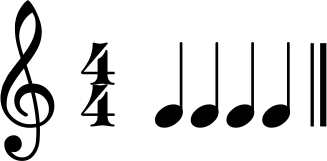
\includegraphics[scale=0.3]{img/discuss1}\\
\end{tabular}
}
}

\subfloat[Parser interpretation.]{
\label{fig:rests:b}
\parbox{0.4\linewidth}{
\Tree
[ .{$\frac{1}{1}$} [ .{$\frac{1}{2}$} [ .{$\frac{1}{4}$} [ .$*$ ] [ .$\bullet$ ] ] [ .{$\frac{1}{4}$} [ .$\bullet$ ] [ .$\bullet$ ] ] ] [ .$\bullet$ ] ] 
}
}
\subfloat[]{
\label{fig:rests:score}
\parbox{0.4\linewidth}{
\begin{tabular}{ l  >{\centering\arraybackslash}m{2in} }
A & 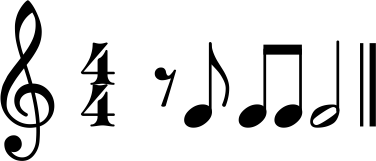
\includegraphics[scale=0.3]{img/discuss2}\\
B & 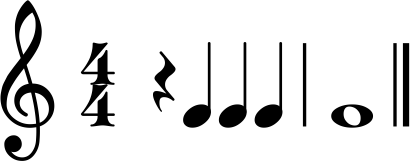
\includegraphics[scale=0.3]{img/discuss3}\\
\end{tabular}
}
}

\parbox{0.4\linewidth}{
\subfloat[A representation that includes rests.]{
\label{fig:rests:c}
\Tree
[ .{$\frac{1}{1}$} [ .{$\frac{1}{2}$} [ .{$\frac{1}{4}$} [ .$*$ ] [ .$\bullet$ ] ] [ .{$\frac{1}{4}$} [ .$\bullet$ ] [ .$\bullet$ ] ] ] [ .{$\frac{1}{2}$} [ .{$\frac{1}{4}$} [ .$\bullet$ ] [ .Rest ] ] [ .Rest ] ] ]
}
}
\subfloat[]{
\parbox{0.4\linewidth}{
\begin{tabular}{ l  >{\centering\arraybackslash}m{2in} }
A & 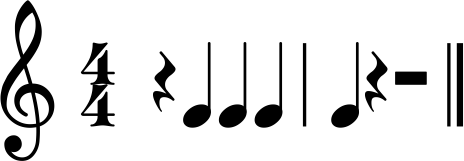
\includegraphics[scale=0.3]{img/discuss4}\\
\end{tabular}
}
}
\caption{An example of why rests are desirable to correctly represent the last note.}
\label{fig:rests}
\end{figure}
